\chapter{Results}

Studies of several emission peaks of neutral Ba in SXe are discussed in \ref{sec:fluorescence}.  Temperature and annealing dependence are discussed in \ref{subsec:tempanneal}, and bleaching of these peaks is discussed in detail in \ref{subsec:bleaching}.  Imaging of Ba fluorescence in a focused laser region is discussed in \ref{imaging}, with the ultimate achievement of imaging at the single atom level using the 619-nm fluorescence peak.  Candidate fluorescence peaks of Ba\textsuperscript{+} in SXe are reported in \ref{sec:BaPlus}.

\section{Fluorescence of Ba in SXe}
\label{sec:fluorescence}

Deposits of Ba in SXe absorb primarily between 540~nm and 570~nm.  An absorption spectrum, obtained by observing absorption of white light by a large Ba deposit at 11~K, is shown in Fig. \ref{fig:BaAbs}, along with an example emission spectrum of a Ba\textsuperscript{+} deposit made at 45~K and observed at 11~K with 557~nm excitation.  Significant broadening, as well as a 4-nm redshift  of the central peak, occur relative to the vacuum $6s^{2}$ $^{1}$S$_{0} \rightarrow 6s6p$ $^{1}$P$_{1}$ absorption value of 553.5~nm.  Initial discovery of this absorption and emission was done with the purely neutral Ba getter source.  Observation of the same spectra from Ba\textsuperscript{+} ion beam deposits demonstrates some neutralization of the ions.  The fraction of ions neutralized is not determined.  \cite{Mong2015,Shon,Brian}

\begin{figure} %[H]
        \centering
                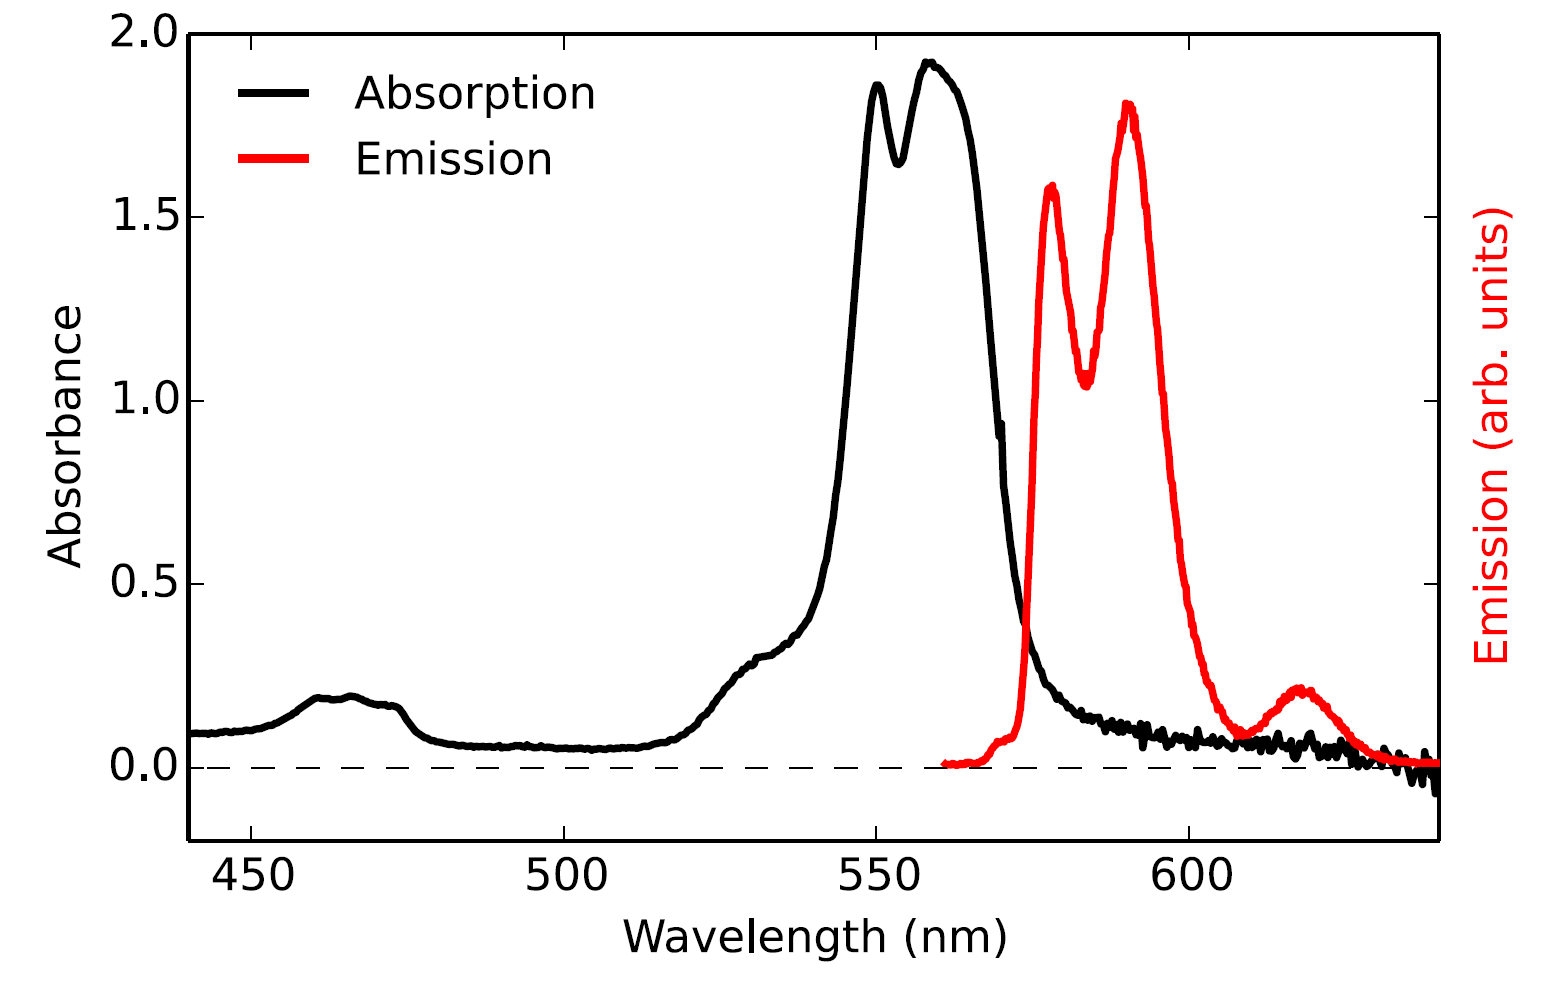
\includegraphics[width=.7\textwidth]{figures/BaAbs_fromBaSpec.png}
                \caption{Absorption and emission spectra of neutral Ba in SXe.  \cite{Mong2015}}
\label{fig:BaAbs}
\end{figure}

\begin{figure} %[H]
        \centering
                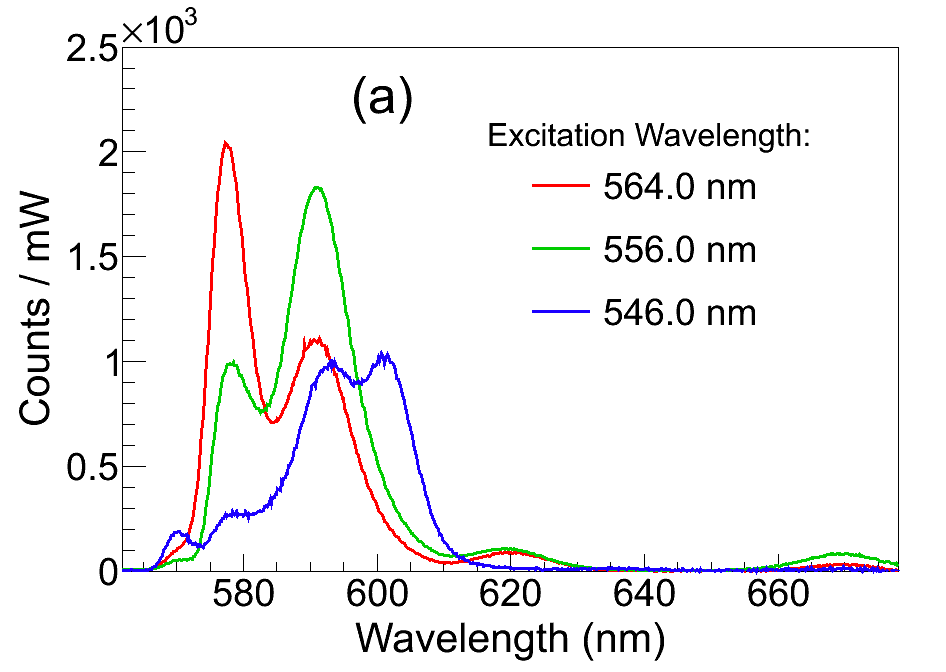
\includegraphics[width=.5\textwidth]{figures/excitspec_grn_spectra_v2.png}
                ~
                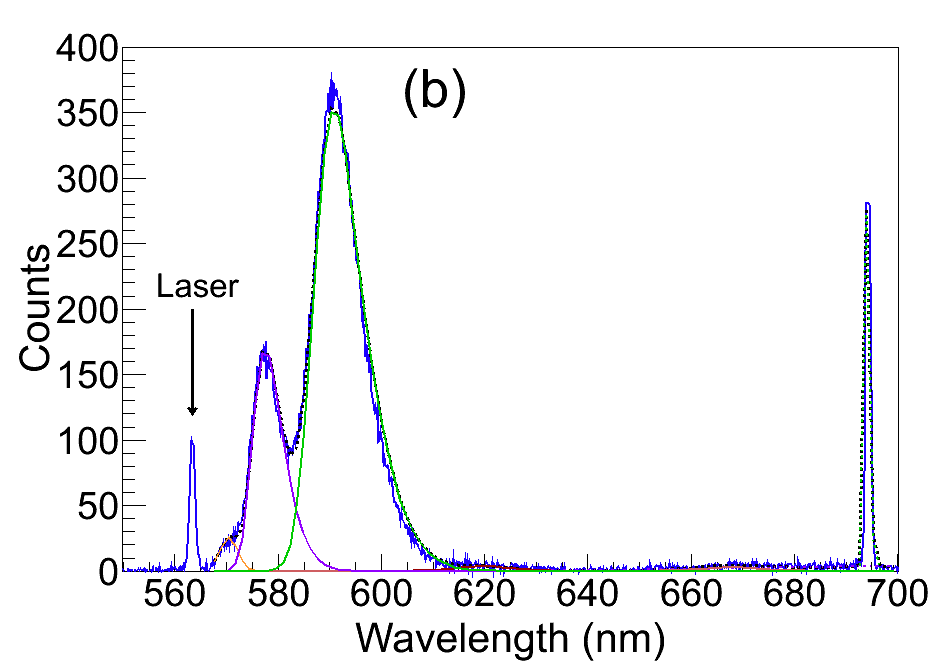
\includegraphics[width=.5\textwidth]{figures/excitspec_grn_spectra_fit.png}
                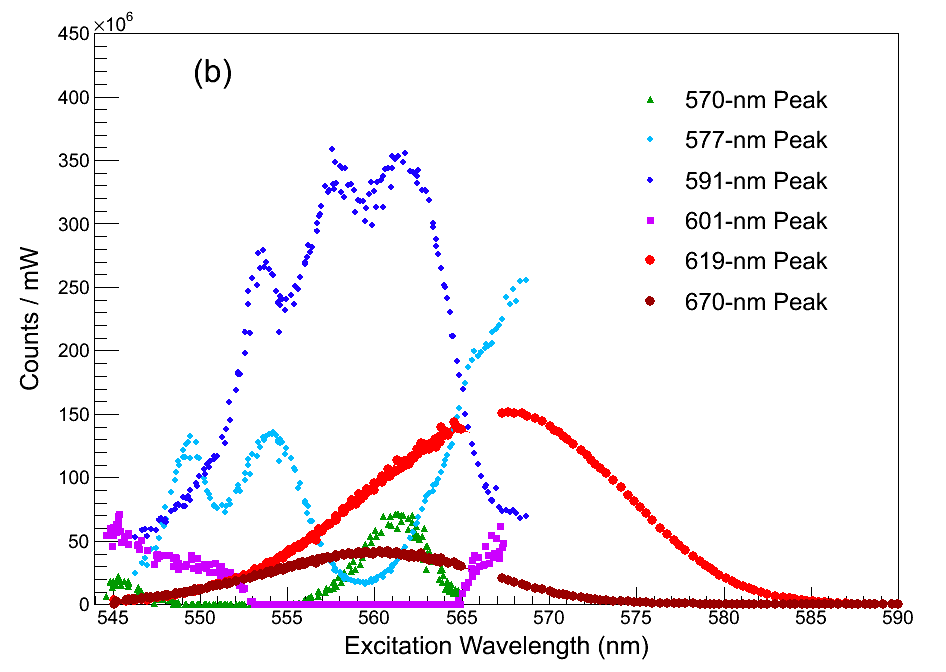
\includegraphics[width=.95\textwidth]{figures/excitspec_grn.png}
                \caption{Background-subtracted fluorescence spectra for a few different excitation wavelengths (a), an example fit to a spectrum (b), and full excitation spectra for all observed Ba fluorescence peaks (c).  Magnitudes in (c) have been scaled for visibility on the same plot (relative magnitudes are arbitrary as they are affected by relative site populations and fluorescence efficiencies).  The discontinuity around 566~nm for the 619- and 670-nm peaks is the boundary between usage of different laser dyes.  R6G dye is used for higher wavelengths and R110 for lower wavelengths and for all other curves.  Curves for the R6G segments (619- and 670-nm peaks) require special scaling to line up with their respective R110 segments, and this scaling was different between the 619- and 670-nm peaks, likely due to different relative populations of those sites on the different deposits.}
\label{fig:excitspecGrn}
\end{figure}

%Put legend in (b)? It's crowded.

%\begin{equation}
%A(1+erf(\frac{x-a}{\sigma_{1}})(1-erf(\frac{x-a}{\sigma_{2}}))
%\label{eqn:specfit}
%\end{equation}

The several red-shifted emission peaks observed are attributed to Ba atoms occupying different matrix sites in the SXe.  Deposition at temperatures higher than 11~K and exploration of more excitation wavelengths have led to discovery of a few emission peaks beyond the 591- and 577-nm peaks reported in \cite{Shon} and \cite{Brian}.  Emission spectra for selected excitation wavelengths are shown in Fig. \ref{fig:excitspecGrn}(a), for a deposit made at 44~K and observed at 11~K.  These selections are part of a full excitation spectrum, shown in Fig. \ref{fig:excitspecGrn}(c).  An excitation spectrum is produced by scanning the dye laser and measuring the magnitude of each fluorescence peak vs. excitation wavelength.  For each 1-s CCD exposure, a sum of asymmetric Gaussian functions and standard Gaussian functions is fit to the spectrum after pedestal subtraction.  The asymmetric Gaussian fit function used, which fits the 577- and 591-nm peaks somewhat better than standard Gaussians, is $A(1+$erf$(\frac{x-a}{\sigma_{1}})(1-$erf$(\frac{x-a}{\sigma_{2}}))$, where $A$ is the free amplitude parameter.  The peak position $a$ is fixed for each peak, as are the left and right smearing widths $\sigma_{1}$ and $\sigma_{2}$.  The function erf() is a Gaussian error function.  The asymmetric Gaussian function is not perfect for all frames, as the shape of the emission can depend on the excitation wavelength.  An example frame with fits is shown in Fig. \ref{fig:excitspecGrn}(b).  The full fit is the dotted black line, and each peak's contribution is in color.  Curves in (a) have about 100$\times$ the laser power used in the excitation spectrum (e.g. (b)) where low intensity is desired to avoid bleaching during the scan.  Rather than attempting frame-by-frame background subtractions, additional Gaussians are fit to the broad and sharp background fluorescence.  These backgrounds and their excitation spectra are discussed in \ref{sec:bgs}.  A 566~nm Raman filter was used to attenuate the majority of the laser scatter, however the small amount of scatter passed by the filter was used to determine the frame's excitation wavelength.  Each peak's fit contribution was then integrated and scaled by the frame's laser power, as the power output is not constant through the dye range.

%\emph{\color{gray}Care about 10~K excitation spectrum?}

Wavelength calibration was done using three lasers whose wavelengths were first measured with a Burleigh Wavemeter:  a red diode laser at 656.99~nm, a doubled Nd:YAG laser at 532.23~nm, and the C480 blue dye laser typically around 475~nm (at 488.91~nm for the data in Fig. \ref{fig:excitspecGrn}).  These lasers were directed at the same position on the sapphire window, and their scatter was imaged along the same path as the Ba fluorescence.  The WinSpec software applies the diffraction grating equation to calibrate each CCD pixel to a wavelength.

\subsection{Annealing/Temperature Dependence}
\label{subsec:tempanneal}

%\emph{\color{gray}When does it need to be mentioned that certain data was also used in the paper(s)?}

Matrix site occupancies for Ba atoms can depend on annealing history, and similarly on the temperature at which a deposit is made.  Spectra under different temperature conditions are shown in Fig. \ref{fig:specTempConditions}.  Peak shapes look similar for deposits made at 40-55~K as those made at 11~K and then annealed to 40-55~K, both being observed at 11~K, though relative amplitudes are not the same, likely due to matrix site populations.  Without annealing, 11-K deposits have a different peak shape around 590~nm, with a broader peak centered around 596~nm.  It is possible that the broader shape is due to a higher population of the 601-nm peak, and it is not resolved from the 591-nm peak.  The experiment in Fig. \ref{fig:specTempConditions} did not have optimal laser intensity for observing behavior of the 619-nm peak; a study of deposit conditions for this peak is shown in Fig. \ref{fig:specTempConditions619}.  In that experiment, the 619-nm fluorescence was observed in a focused laser beam at 570~nm, in an image through the 620-nm band-pass filter.  About 3$\times$ more 619-nm fluorescence was observed in the deposit at 52~K vs. 11~K for the same leak rate (the respective 31~nm/s and 37~nm/s are from the same Xe leak rate, resulting in different SXe deposition rates daccording to Fig. \ref{fig:fringes_52K_vs_11K}).  Also in this figure is a deposit at 11~K with the lower leak rate resulting in about 5~nm/s SXe deposition, which produced nearly 3$\times$ lower signal than the leak rate resulting in 37~nm/s SXe deposition.  Using the 10~K SXe density of 3.780~g/cm\textsuperscript{3} \cite{SXeDensity} and a typical Ba\textsuperscript{+} ion current density of 1.6~nA/mm\textsuperscript{2} at the sapphire window, 5~nm/s and 37~nm/s correspond to Xe:Ba ratios of about $8.7 \times 10^{3}$ and $6.4 \times 10^{4}$ respectively.  \emph{\color{gray}This difference spans the threshold of $10^{4}$ recommended in (cite? refer to Ch.2?) for isolated guest atoms (still italic because it depends on what you quote in Ch.2).}   Xe leak rates above 37~nm/s result in rapid frosting of the SXe matrix, which causes blurring of the image and high laser scatter.  These tests guided the standard of depositing with Xe leak rate resulting in 31~nm/s SXe deposition at 50$\pm$5~K when observing the 577-, 591-, and/or 619-nm peaks.  The different bleaching behavior in the low Xe leak rate deposit is discussed in \ref{subsec:bleaching}.

%keyword barfbreath for above reference to the Ba:Xe ratio mention in Theory

%5.4E4 Xe:Ba for leak 48 50~K (31 nm/s)

\begin{figure} %[H]
        \centering
                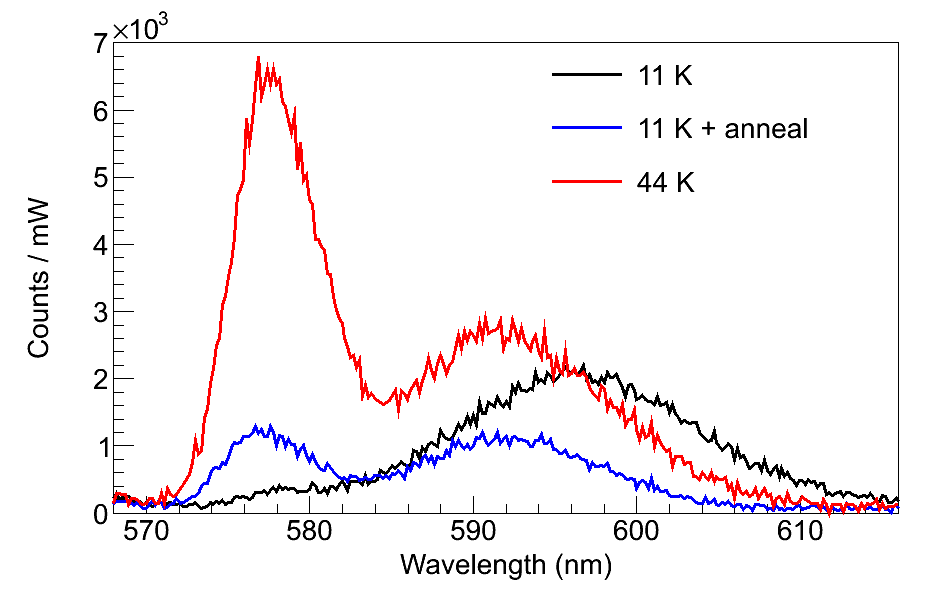
\includegraphics[width=.7\textwidth]{figures/spectra_temperature_conditions.png}
                \caption{Spectra of peaks around 590~nm of a Ba\textsuperscript{+} deposit made at 11~K before and after annealing to 39.4~K, and one made at 44~K.  All observations are at 11~K.  Both Ba\textsuperscript{+} deposits are 15~s, however the 44~K deposit is scaled slightly to account for different ion current.  Laser power was about 0.1~mW with an unfocused beam waist of w = 7.056~mm, at 566~nm wavelength.}
\label{fig:specTempConditions}
\end{figure}

\begin{figure} [h]
        \centering
                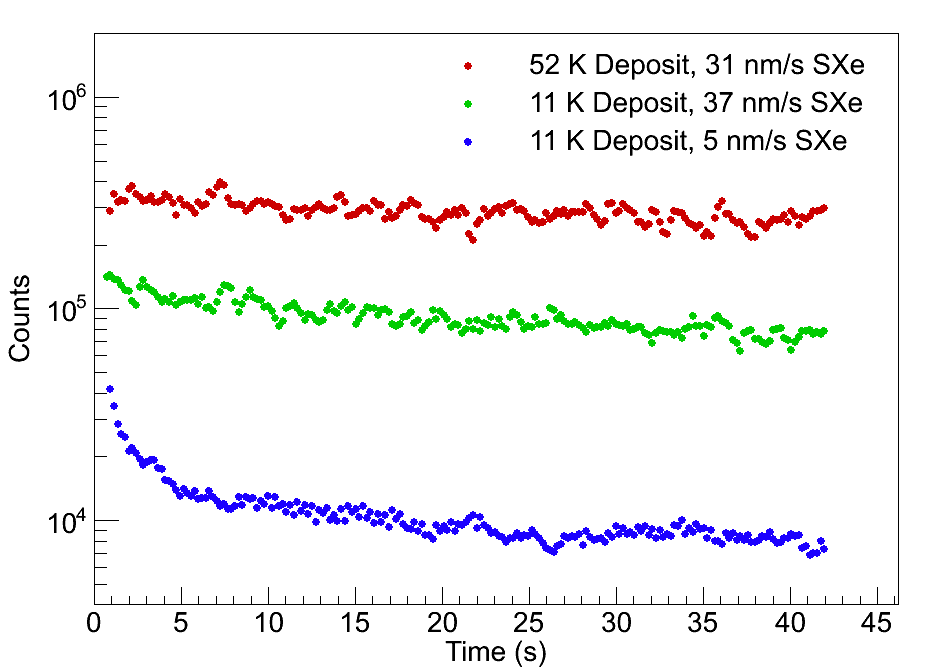
\includegraphics[width=.7\textwidth]{figures/619_deposit_conditions.png}
                \caption{Summed 619-nm fluorescence counts over time from imaging focused 570-nm laser region, for Ba\textsuperscript{+} deposits at different temperature and Xe leak conditions.  Frame times are 0.1~s, with time in between frames of about 0.11~s.}
\label{fig:specTempConditions619}
\end{figure}

\begin{figure} %[H]
        \centering
                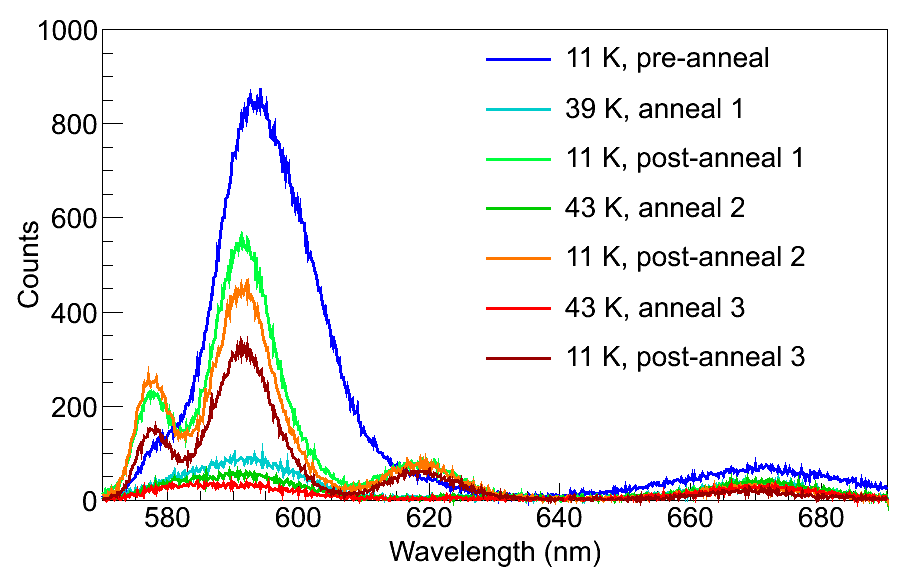
\includegraphics[width=.95\textwidth]{figures/spectra_annealing.png}
                \caption{Spectra of a large Ba\textsuperscript{+} deposit through several annealing cycles.  Initial deposit was at 11~K.  Laser power was about 0.2~mW with an unfocused beam waist of w = 7.056~mm, at 564~nm wavelength.  These are selections from the full data set shown as peak counts vs. temperature in Fig. \ref{fig:annealGrn}.  \emph{\color{red}This same data, but a different plot, is in BaSpec, as is some of the annealing plots -- do I just cite the paper or what?} \emph{\color{blue}rm things like that and write them in blue w/ pen on printout}}
\label{fig:specAnneal}
\end{figure}

Fluorescence spectra with 564~nm excitation through several annealing cycles for a deposit made at 11~K are shown in Fig. \ref{fig:specAnneal}.  At this wavelength, all observed Ba peaks are prominent except the 570-nm peak.  Similar to excitation spectra, individual fluorescence peak amplitudes can be plotted vs. temperature by fitting the full spectrum in each frame.  Rather than asymmetric Gaussians, this analysis used standard Gaussian and Lorentzian functions.  Lorentzians fit the 619-nm and 670-nm peaks well.  Each individual peak's amplitude is plotted vs. temperature in Fig. \ref{fig:annealGrn}(b-f), with an example of a fit spectrum in Fig. \ref{fig:annealGrn}(a).  In this interpretation, the 601-nm peak along with the 591-nm peak fit the broader peak in the initial 11~K deposit.  The 601-nm peak had nearly complete loss in the first anneal cycle.  The 670-nm peak had significant loss, with more loss after each succeeding anneal cycle, each of which reached higher a temperature than the last.  The 591-nm had moderate loss with each cycle.  The 577-nm and 619-nm peaks gained significantly with the first anneal, suggesting that they are due to more stable matrix sites.  Both peaks remained about the same after the second cycle (small gain in 577-nm), and both had loss after the third cycle, which reached the higher temperature of 48~K. This could be due to greater diffusion at higher temperature leading to Ba/Ba interactions \emph{\color{gray}ref?}.

\begin{figure} %[H]
        \centering
                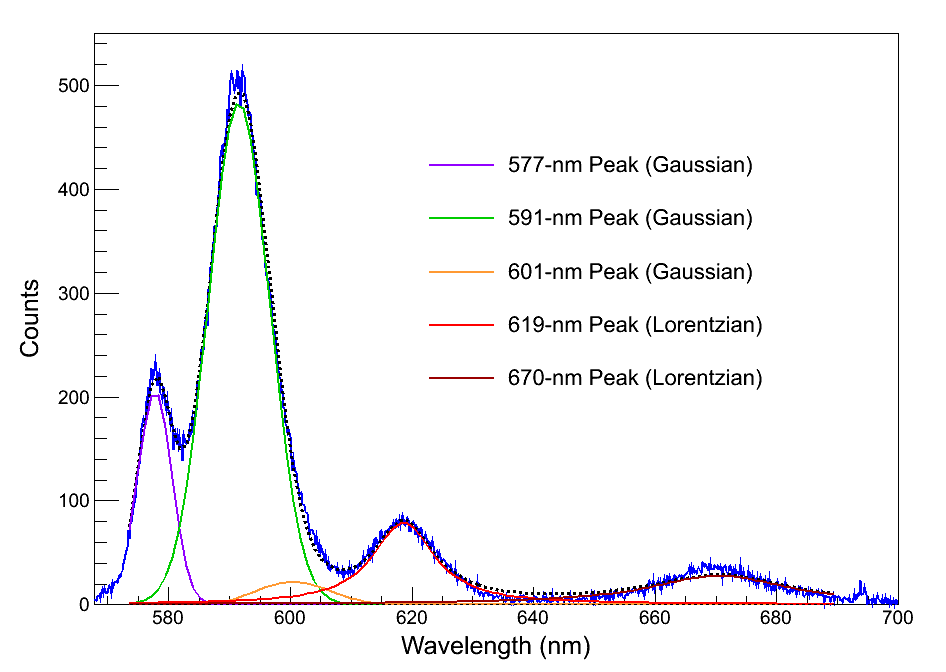
\includegraphics[width=.5\textwidth]{figures/spectra_anneal_fit.png}
                ~
                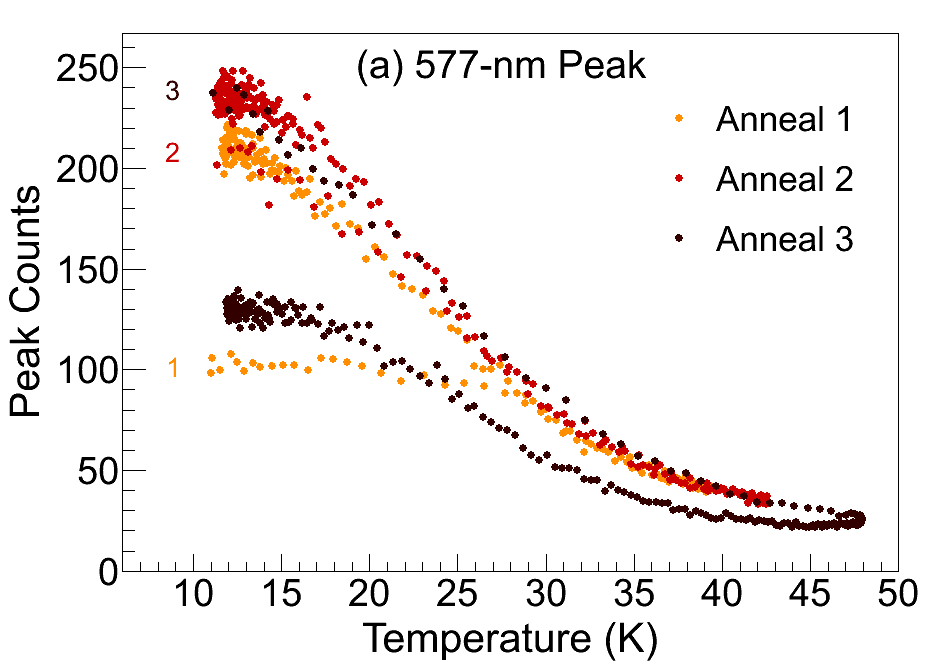
\includegraphics[width=.5\textwidth]{figures/anneal_577peak.png}
                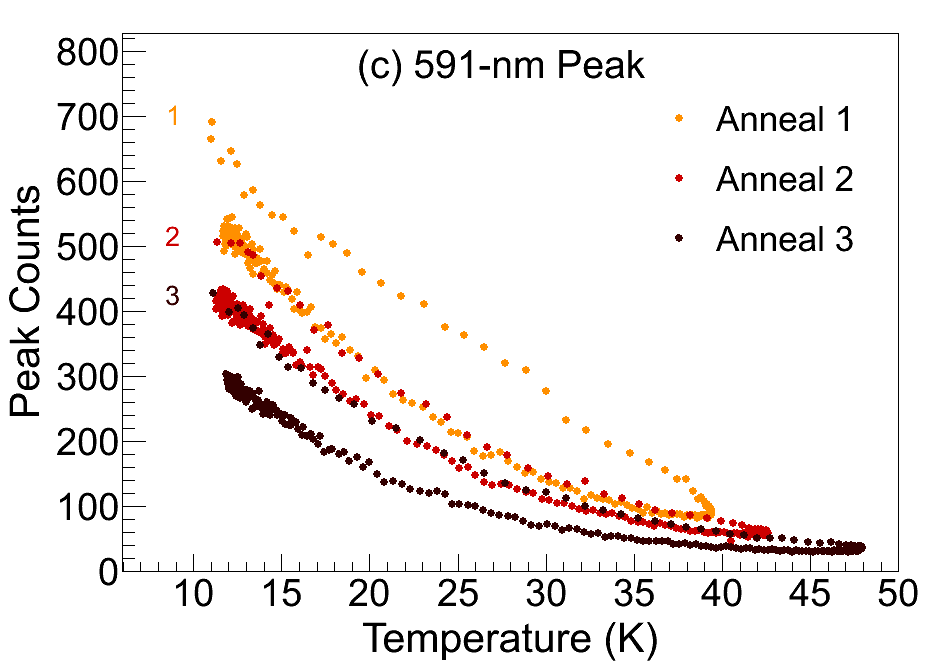
\includegraphics[width=.5\textwidth]{figures/anneal_591peak.png}
                ~
                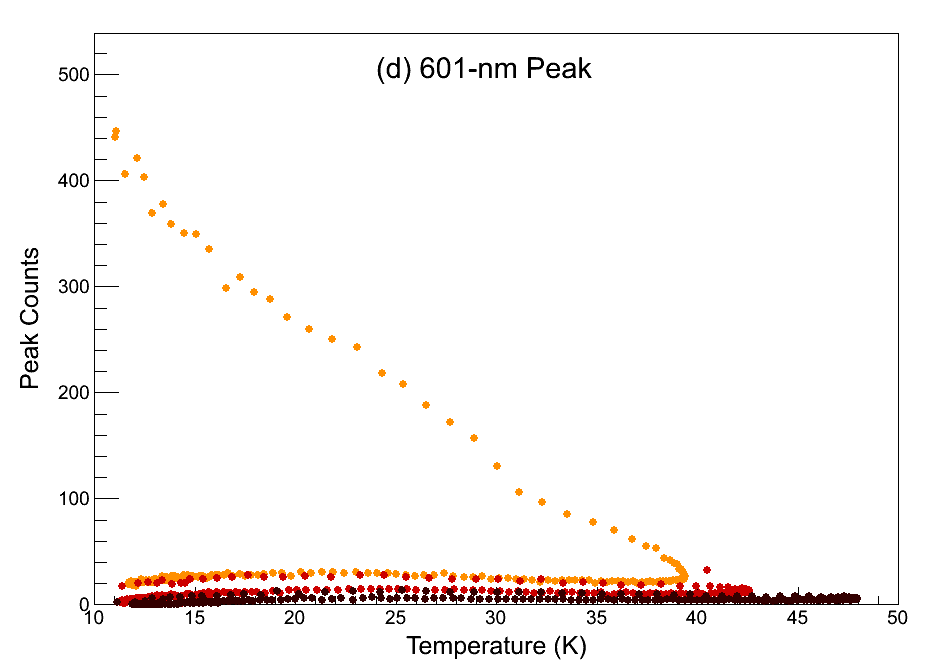
\includegraphics[width=.5\textwidth]{figures/anneal_601peak.png}
                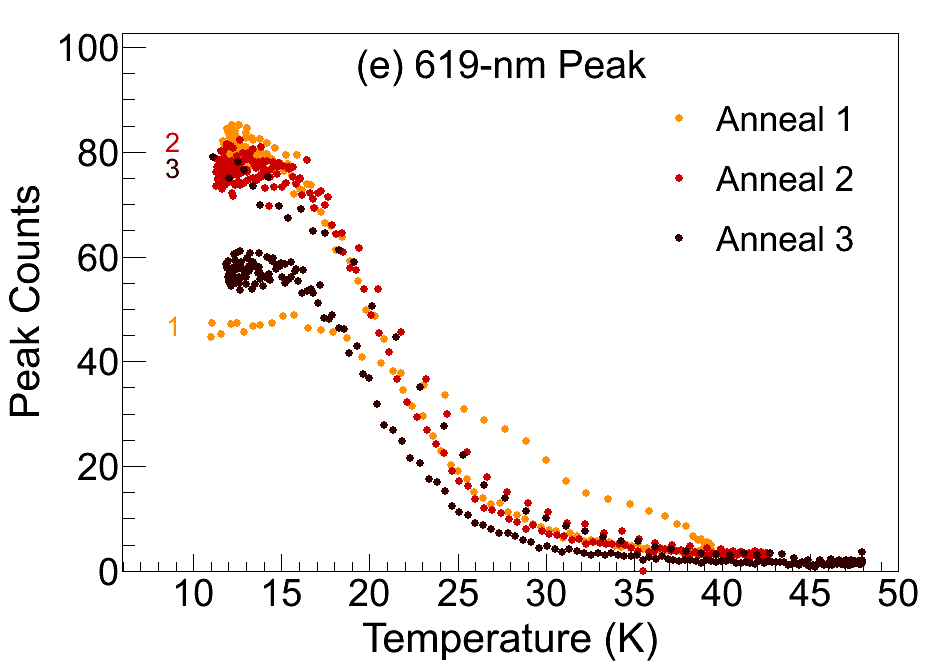
\includegraphics[width=.5\textwidth]{figures/anneal_619peak.png}
                ~
                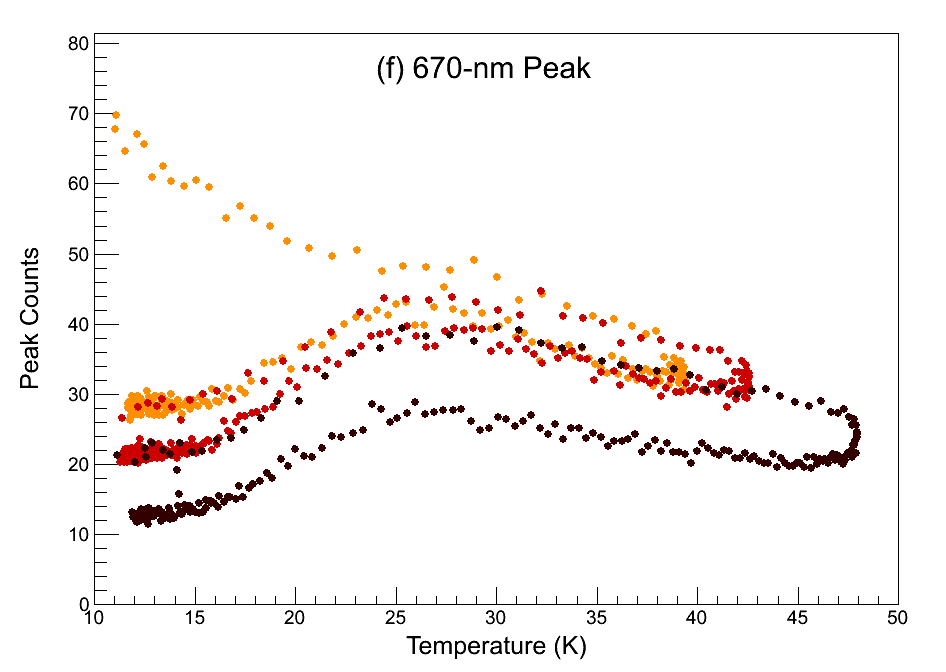
\includegraphics[width=.5\textwidth]{figures/anneal_670peak.png}
                \caption{Example fit with standard Gaussians and Lorentzians (a) and fit peak counts for each fluorescence peak through three annealing cycles of the Ba\textsuperscript{+} deposit made at 11~K (b-f).  ``1, 2, and 3" mark the beginning of each anneal cycle.  Laser power was about 0.2~mW with an unfocused beam waist of w = 7.056~mm, at 564~nm wavelength.}
\label{fig:annealGrn}
\end{figure}

Aside from matrix site changes, direct temperature dependence of fluorescence can be observed in annealing cycles.  The 577-, 591- and 619-nm peaks have their highest amplitude at 11~K.  The 577-nm and 619-nm peaks appear to be leveled off at 11~K, while the 591-nm may benefit from even lower temperatures.  The 670-nm peak has its highest amplitude at around 25~K (apparent after its major site alteration has occurred).  This inverse relationship between fluorescence and temperature suggests that a probe in nEXO will need to be moved to an evacuated chamber in order to cool to 11~K or below for observation.  

%\emph{\color{gray}601 and (not shown) 570 would require different wavelength to study.}

%[inverse relationship] could be due to a different matrix environment at higher temperature, or possibly a loss of fluorescence efficiency due to increased non-radiative decays from the excited state.  

\subsection{Bleaching}
\label{subsec:bleaching}

\emph{\color{gray}This section is referred to in annealing section as talking about different bleaching in leak 44 runs.}

Decay of fluorescence with laser exposure, or bleaching, was observed for all six Ba fluorescence peaks.  It is a rapid process for the 570-, 577-, 591-, and 601-nm peaks, and a much slower process for the 619- and 670-nm peaks.  With the prospect of counteracting the effect for single-atom imaging, bleaching of the 577- and 591-nm peaks was studied in detail by observing the fluorescence decay rate for varying excitation rates.  

To produce a well-known laser intensity, the laser was de-focused to a specific beam waist (w), and the image of 619-nm fluorescence (which defines the laser region due to its low bleaching) from a large Ba\textsuperscript{+} deposit was centered in the spectrometer slit and a y-pixel region of interest (ROI) with edges at 90\% of the maximal intensity.  Fluorescence counts vs. time \emph{\color{gray}(excitations?)} for the 577- and 591-nm peaks are plotted in Fig. [fig bleaching].  \emph{\color{gray}...explain... does it make sense?} ({\color{red}do a correction on p-meter sensitive area and on p-meter quantum efficiency, and also a spherical aberation correction for power, though that may not matter for the defocused studies.})

590 etc, model fit -- they look like vacuum rates

%\begin{figure} %[H]
 %       \centering
  %              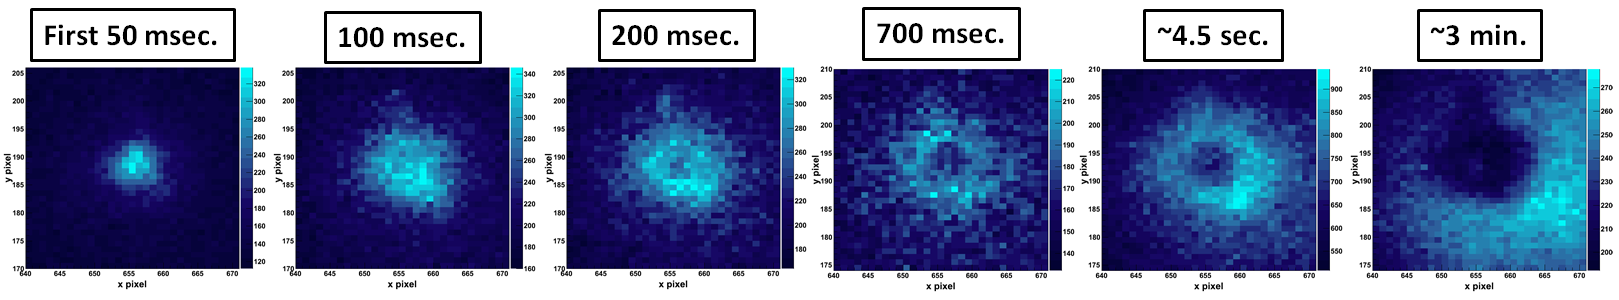
\includegraphics[width=.9\textwidth]{figures/hole_bleach_590.png}
   %             \caption{}
%\label{fig:testfig}
%\end{figure}

Effecting re-pumping of optically pumped Ba could require up to three additional lasers, one for each of the populated metastable D states, as it does in vacuum.  The optimal absorption for each transition would need to be discovered using tunable lasers in the infrared, and the search would be challenging, as the effect of re-pump is small until all three are achieved.  However, mixing of states in the Xe matrix could lower the number of lasers needed.  Searches for an effect of additional excitation lasers were attempted with a few different lasers.  \emph{\color{red}describe which lasers were supposed to do which transitions -- 1550, 1064, 657, 406, blue bye}.

The only effects observed on bleaching rates by these re-pump lasers were increased bleaching by the blue dye and 406-nm Kr ion lasers.  Some effect of a return of fluorescence was observed for separate exposures of low-intensity 406-nm Kr ion laser, shown in Fig. [fig Kr return].  In this experiment, bleaching of the 591-nm peak was observed by x-nm excitation, and then the x-nm laser was blocked for a length of time, either for a waiting period or for exposure to the 406-nm laser.  Larger returns in 591-nm fluorescence were observed with 406-nm exposure than for just waiting, for low intensities of the 406~nm.  However, co-exposure of this intensity of 406~nm with the green excitation laser had no noticeable effect.  This phenomenon was not explored further.

Another possible mechanism for bleaching is matrix site change caused by the difference in the Ba-Xe interactions when the Ba is in the excited state.  This was explored in an experiment where excitation spectra were produced before and after bleaching the Ba sample at various wavelengths.  Selected runs are shown in Fig. [bleaching excitspec].  \emph{\color{gray}describe -- interesting changes may reveal different site components of the peaks -- or does it?  idk how this could happen ... cuz the triple peak thing was supposedly normal for a single site ... small rises were ween, but poplulations cannot be known, so we don;t know}

The 619-nm peak bleaches at much higher laser intensities, only becoming a limiting factor in a focused laser at \emph{\color{red}several?} mW.  619-nm fluorescence vs. time from an image in a focused laser at x~nm for three laser powers.  ... defines power we use

\section{Backgrounds}
\label{sec:bgs}

One source of background emission was observed from the surfaces of the window.  Its broad fluorescence is shown in Fig. \ref{fig:surfBG}(a) with a 610-nm Raman filter cutoff and 570.4~nm excitation, and its excitation spectrum is shown in Fig. \ref{fig:surfBG}(b) over the R6G dye range.  The nature of this emission has not been determined, however a few features were identified.  One was that the emission increased as the window temperature was decreased, down to about 100~K where it remained flat down to 11~K, shown in Fig. \ref{fig:BGtempDependence}.  Another feature of the surface background is that it bleaches with laser exposure.  This was useful in that the background could be reduced by pre-bleaching of the window.  However, the bleaching behavior also presented an inconvenient time dependence of the surface background, as historical bleaching and possible slight movements of the laser could lead to variation.  Frequent Xe-only deposits were made in order to establish proper background subtraction.  Spacial variation in the background is especially cumbersome in a laser scanning experiment, as discussed in \ref{sec:scanning}.  Given these behaviors, it is possible that the surface background is caused by a species which freezes to the window, or something which coats the window and fluoresces more at lower temperatures.  In either case, the bleaching could be explained by evaporation with laser heating, or by optical pumping of the species into a metastable state.

%, shown in Fig. [fig surfaceBG bleaching]

\begin{figure} %[H]
        \centering
                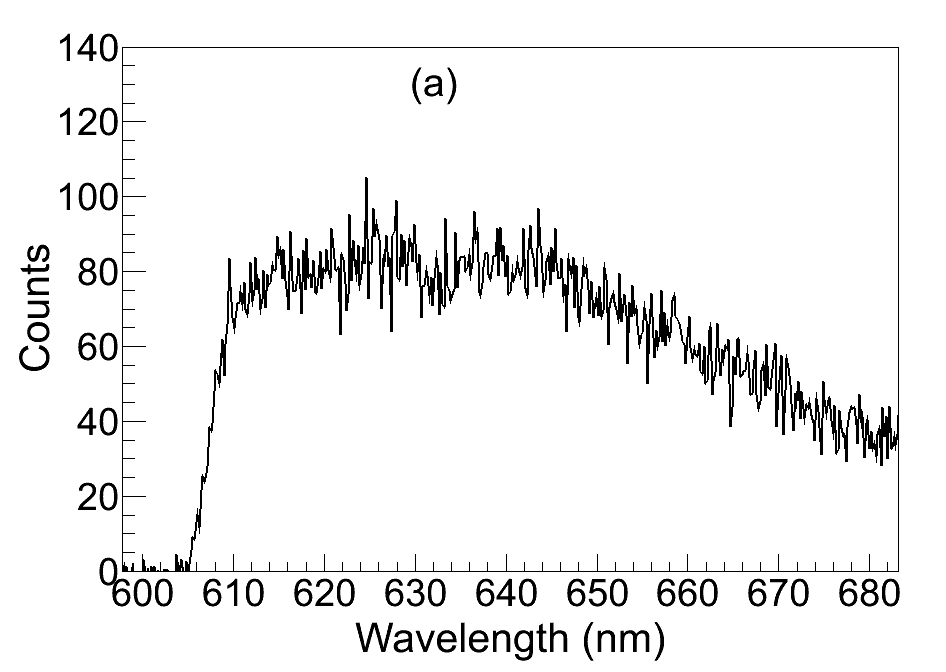
\includegraphics[width=.7\textwidth]{figures/surfaceBG_a.png}
                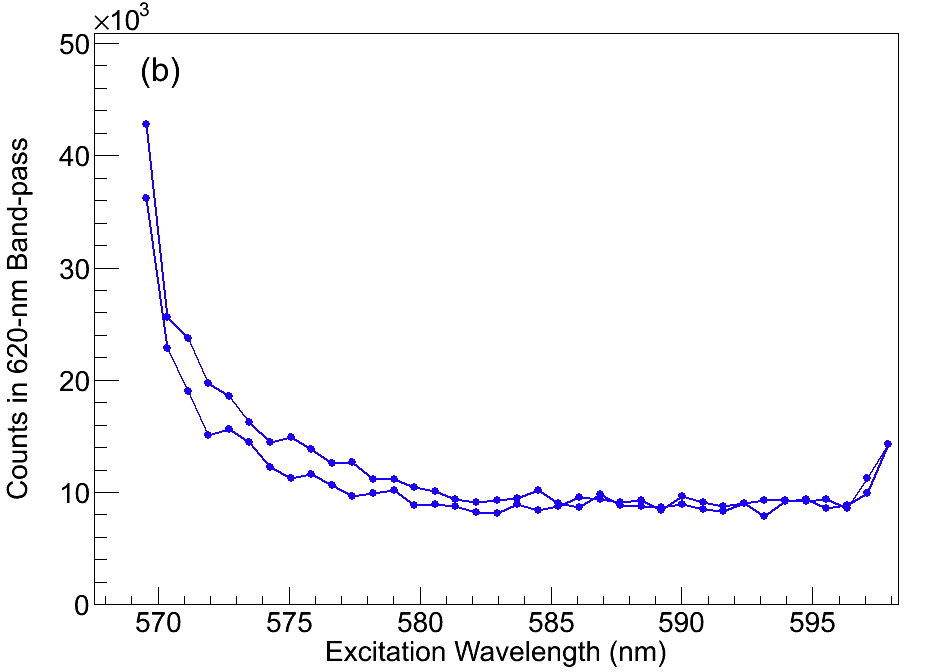
\includegraphics[width=.7\textwidth]{figures/surfaceBG_b.png}
                \caption{Surface background emission spectrum w/ excitation at 570.5~nm (a) and its excitation spectrum in R6G dye range (b).  The sharp drop in (a) around 608~nm is the Raman filter cutoff.}
\label{fig:surfBG}
\end{figure}

\emph{\color{red}Plz uncomment the following after the figure exists:}
%\begin{figure} %[H]
%        \centering
%                \includegraphics[width=.7\textwidth]{figures/BG_T-dependence.png}
%                \caption{}
%\label{fig:BGtempDependence}
%\end{figure}

\begin{figure} %[H]
        \centering
                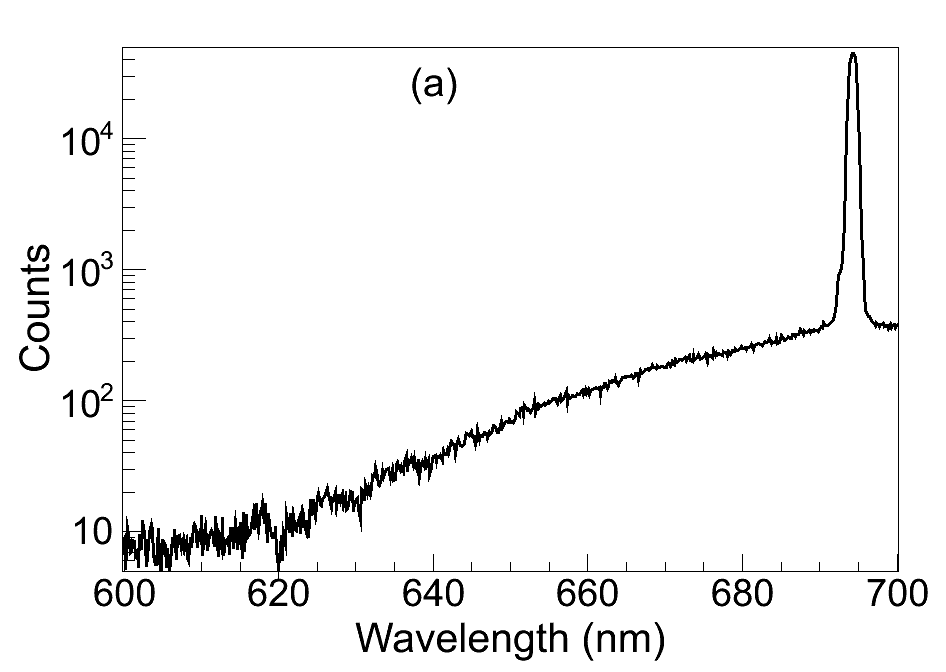
\includegraphics[width=.7\textwidth]{figures/Cr_a.png}
                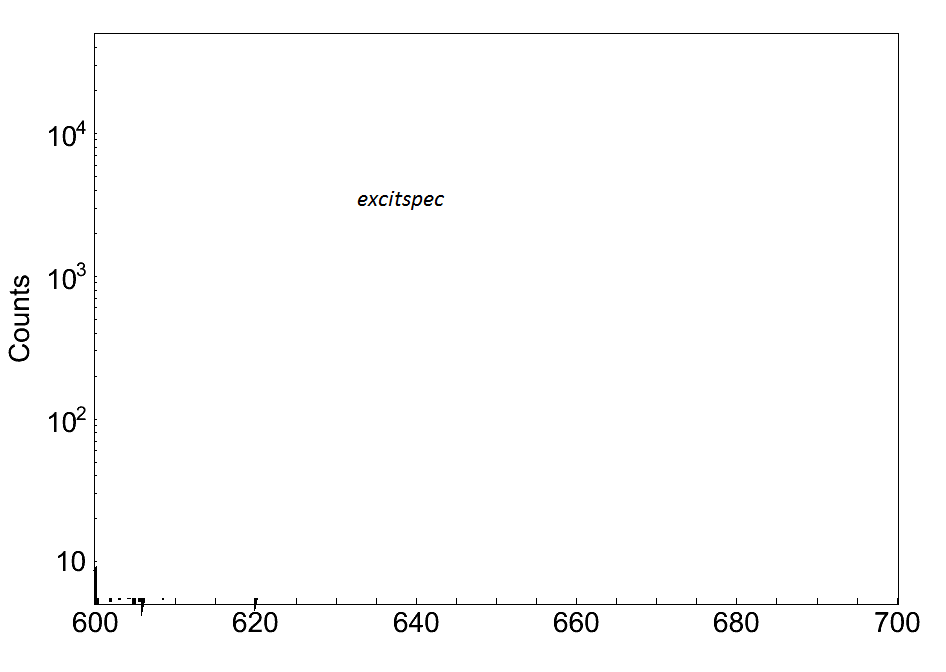
\includegraphics[width=.7\textwidth]{figures/Cr_b.png}
                \caption{562-nm excitation, 11~K.  Say not seen is another peak which is only at like 100 K and up?}
\label{fig:Cr}
\end{figure}

\begin{figure} %[H]
        \centering
                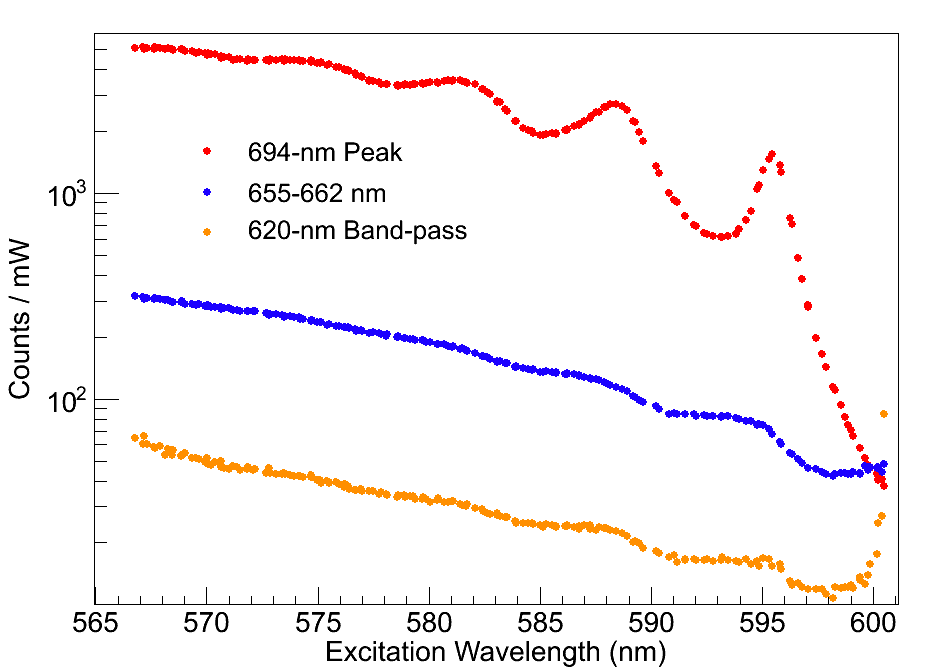
\includegraphics[width=.7\textwidth]{figures/Cr_broad.png}
                \caption{}
        \label{fig:CrBroad}
\end{figure}

Another source of background is fluorescence from the sapphire window.  A spectrum of this fluorescence with 562~nm excitation is shown in Fig. \ref{fig:Cr}(a).  The strong, sharp peak at 694~nm is a well-known emission of Cr\textsuperscript{3+} impurities in the sapphire bulk.  An excitation spectrum for this peak is shown in Fig. \ref{fig:Cr}(b) over the range all three dyes R6G, R110, and C480, using a sapphire window with relatively high Cr\textsuperscript{3+} content.  Multiple features observed in the excitation spectrum are consistent with the absorption spectrum of Cr\textsuperscript{3+} in sapphire at 77~K, including three sharp peaks in the blue, and a broad absorption in the green/yellow with vibrational peaks on the red tail \cite{SapphireFord,SapphireMcclure}.  In addition to the 694-nm peak, a weaker and much broader emission is observed, along with three weak peaks around the 619-nm Ba peak region, also from the sapphire bulk.  Excitation spectra for these fluorescence components are shown in Fig. \ref{fig:CrBroad} for the R6G dye range.  In this experiment, the laser was de-focused to about w = 200~$\mu$m, and the emission observed was from the surface laser spot.  As a result, \emph{\color{red}need to say that surface BG comes in on weak parts of the Cr emission ... it's the same experiment as other figure} Observation of the same vibrational peaks demonstrates that this emission is also due to Cr\textsuperscript{3+} in the sapphire.  Commercially available c-plane quality sapphire windows contain very low concentrations of Cr\textsuperscript{3+}.  Windows from a few companies were tested, and those from Meller Optics produced the lowest sapphire bulk emission in the 620-nm band-pass region.  The choice of 570~nm for excitation of the 619-nm fluorescence peak was made by an optimization of $S$/$\sqrt{B}$, where $S$ is the 619-nm signal and the background $B$ is the broad emission in the 620 band-pass filter region (orange curve in Fig. \ref{fig:CrBroad}).  The Cr\textsuperscript{3+} emission has an inverse relationship with temperature, shown in Fig. \ref{fig:BGtempDependence}.

%with Cr\textsuperscript{3+} concentrations of around {\color{red}10 ppt} observed.

%(peaks around? May need to ask Bill about what peaks exist and at what temps ... a new idea is to just leave it vague, as ``peaks" since you're sure there are at least 2, but vauge is OK)

\section{Imaging}
\label{imaging}

Though the imaging spectrometer can produce spacial images with the 0-order grating reflection, better collection efficiency and imaging quality are achieved by removing the spectrometer and imaging directly onto the CCD.  Band-pass filters were used to pass the desired Ba fluorescence peak(s) while attenuating laser scatter and sapphire fluorescence.

%angle=90,
\begin{figure} %[H]
        \centering
                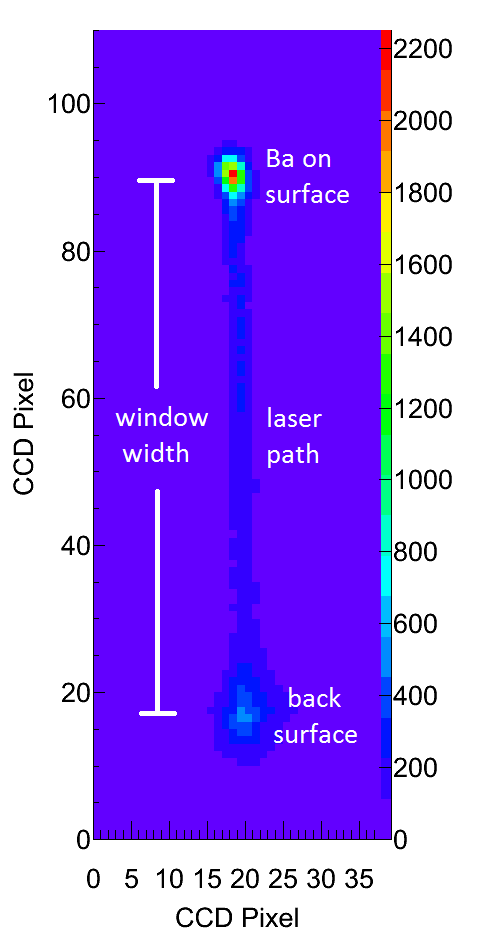
\includegraphics[width=.4\textwidth]{figures/raw_14-atom_labels_from_paper_1f.png}
                \caption{Did you want one with no Ba in it?  It sort of says that.}
\label{fig:imageexamp}
\end{figure}

An example image of the focused 570~nm dye laser passing through a c-plane sapphire window of thickness 0.5~mm, using the 620-nm band-pass filter on the fluorescence, is shown in Fig. \ref{fig:imageexamp}.  With 4$\times$ magnification, each pixel is 5~$\mu$m$\times$5~$\mu$m.  The laser's path through the window is faintly visible by the tail of the broad Cr\textsuperscript{3+} fluorescence in the 620-nm band-pass.  The laser is focused at the top surface of the window, which faces the ion beam.  The surface background is seen on both surfaces.  The observed size of the laser spot, with a 1/e$^{2}$ radius of about 12~$\mu$m, is larger than the 2.06~$\mu$m $\times$ 2.66~$\mu$m 1/e$^{2}$ laser spot size.  Aberrations and vibrations in the collection optics could contribute to this inability to reach the diffraction limit in imaging.

%\begin{wrapfigure}{r}{0.5\textwidth}
  %\begin{center}
   % 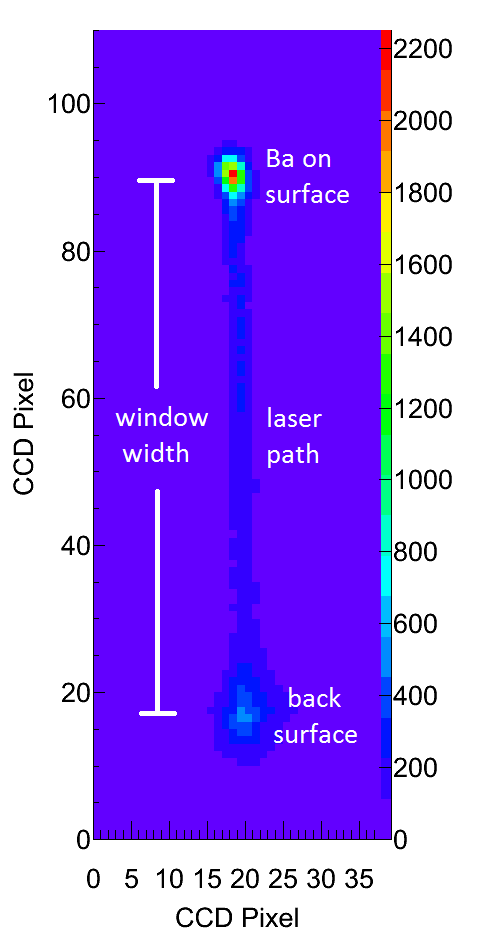
\includegraphics[width=0.35\textwidth]{figures/raw_14-atom_labels_from_paper_1f.png}
  %\end{center}
  %\caption{}
  %\label{fig:imageexamp}
%\end{wrapfigure}

\subsection{Vibrations and Effective Laser Region}

\begin{figure} %[H]
        \centering
                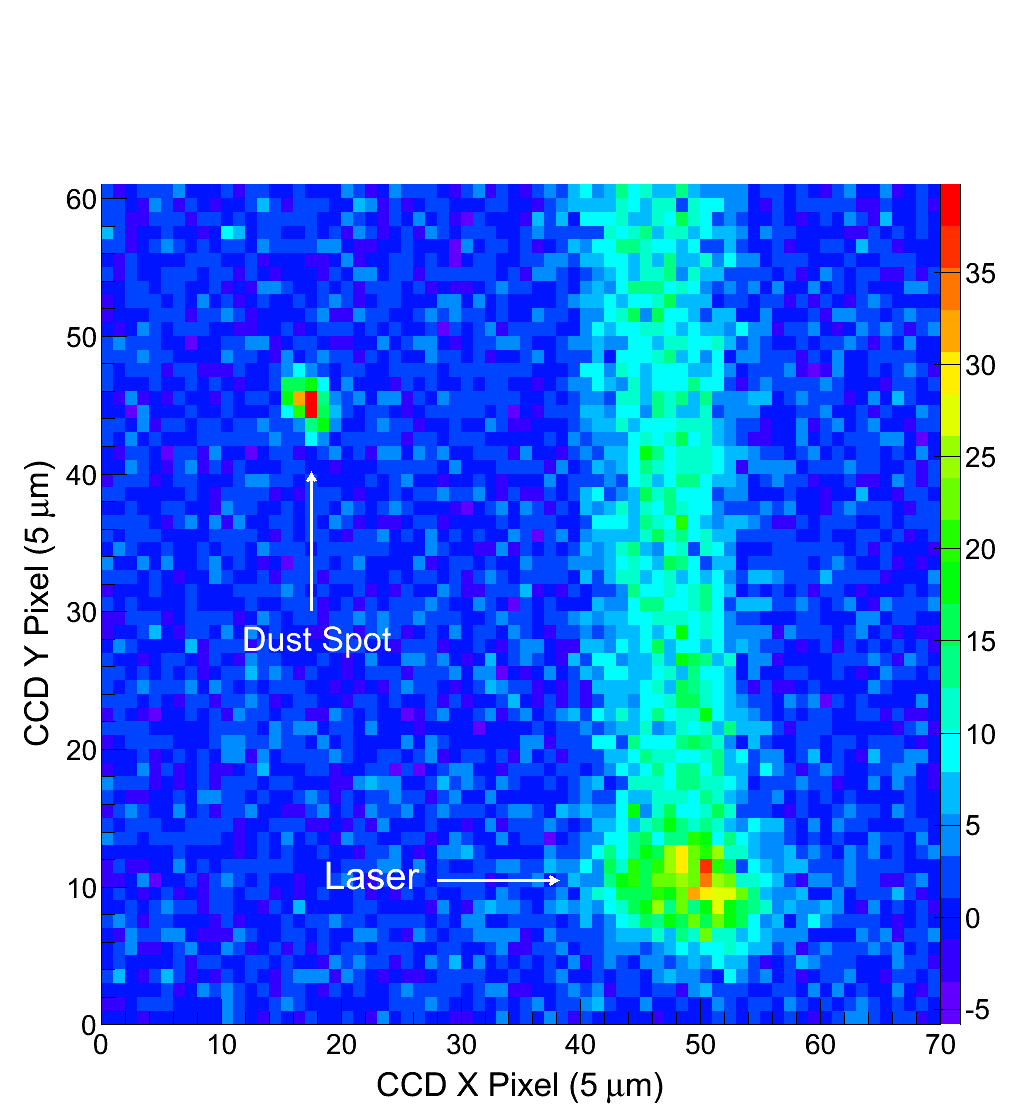
\includegraphics[width=.6\textwidth]{figures/image_dustspot.png}
                \caption{}
\label{fig:dustspot}
\end{figure}

Relative vibrations between the laser and sapphire window will affect the number of Ba atoms exposed, increasing the effective laser spot size.  This was studied by observing the position of a ``dust spot" (a highly scattering feature on the sapphire window) relative to the position of the laser in an image on time scales down to 50~ms.  An example of an image from this experiment is shown in Fig. \ref{fig:dustspot}.  The 570-nm dye laser was somewhat de-focused, and the dust spot was illuminated by a de-focused 657~nm diode laser. For each frame, 2D Gaussian functions were fit to locate the center of the laser spot and the dust spot in order to measure their relative position.  The fit for the laser spot was restricted in y so that it was not affected by the bulk sapphire fluorescence path.  \emph{\color{gray}The difference between dust spot and laser positions is plotted in Fig. [fig vibe vs. time with sine fit] for both x and y.  Each exposure in this plot is 50~ms, though readout time and camera shutter compensation time result in x~s between frames.  The best fit of a sine function results in a vibration frequency of x~Hz.  This is consistent with the audible frequency of the cryostat He pump.}

\emph{\color{red}cryo-vibe figures.}

To calculate an effective laser spot size due to this vibration, each difference (x,y) between laser and dust spot was used as the center of a 2D Gaussian, each with w$_{x} = 2.06~\mu$m and w$_{y} = 2.66~\mu$m to represent the laser spot.  Such Gaussian functions were summed to all points to produce a distribution of summed laser exposure, shown in Fig. [fig vibe sum 2D].  The total area enclosed by a 1/e contour then represents the effective area.  Since x and y movement are correlated, and since the movement is sinusoidal, the effective area is only about 2$\times$ the real laser spot size, and the effective laser region is 17.8~$\mu$m$^{2}$.

The aforementioned is the most concerning vibration to understand.  Vibration of the laser itself is included in that study.  Vibration of the collection optics will affect the imaging resolution, but not the number of atoms being observed.  These vibrations were minimized by stable mounts.

\subsection{Imaging 577- and 591-nm peaks}

\begin{figure} %[H]
        \centering
                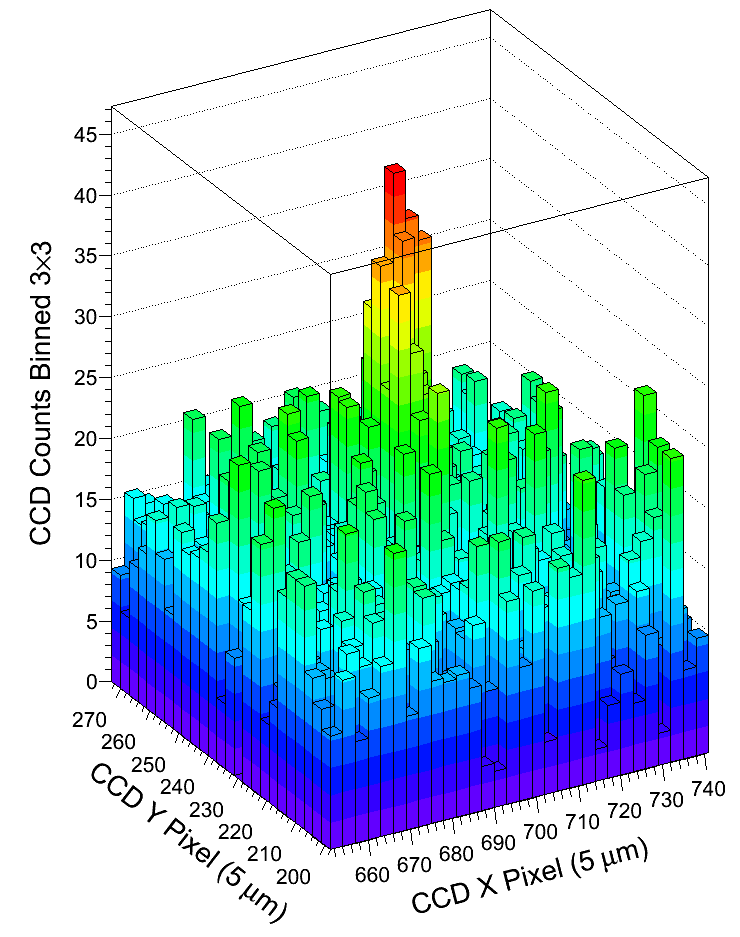
\includegraphics[width=.6\textwidth]{figures/image_1e4.png}
                \caption{\emph{\color{gray}Binned 3x3.  No bleaching at this intensity*t $\rightarrow$ successive frames are not shown.... this is 1e4 total exposed, but basically 5e3 at a given time, and since there's no bleaching maybe that can be quoted.}  \emph{\color{red}Mention ``at one time" thing, which puts the 2.4 to 1 atom.}}
\label{fig:image590s}
\end{figure}

\emph{\color{red}Mention ``at one time" thing, which puts the 2.4 to 1 atom.}  First attempts at imaging small numbers of Ba atoms in a focused laser region were done with the 577- and 591-nm Ba fluorescence peaks together using a 586-nm band-pass filter, which passes 573 - 599~nm FWHM.  This filter has a 2" diameter, resulting in a factor of 4$\times$ more collection efficiency.  Bleaching data was used to optimize laser intensity and exposure time to achieve maximal signal in frame 1, and to avoid hole bleaching.  The fast bleaching of these peaks is the limiting factor on sensitivity.  An image of $\leq$ 10$^{4}$ \emph{\color{gray}Say 5e3? see fig caption} atoms (10$^{4}$ Ba\textsuperscript{+} ions deposited into the effective laser region) is shown in Fig. [fig 590-lines image].  \emph{\color{red}No:} At only x total counts, this is near the limit of sensitivity.  As discussed in [bleaching section], detection of very small numbers of atoms in these sites may require several infrared re-pump lasers.  As a result of low total exposure, neither the sapphire nor the surface backgrounds are present in these images \emph{\color{gray}(but it is Xe-subbed anyway)}.  \emph{\color{gray}talk about long esposure, idk...}

\subsection{Imaging 619-nm peak}

\begin{figure} %[H]
        \centering
                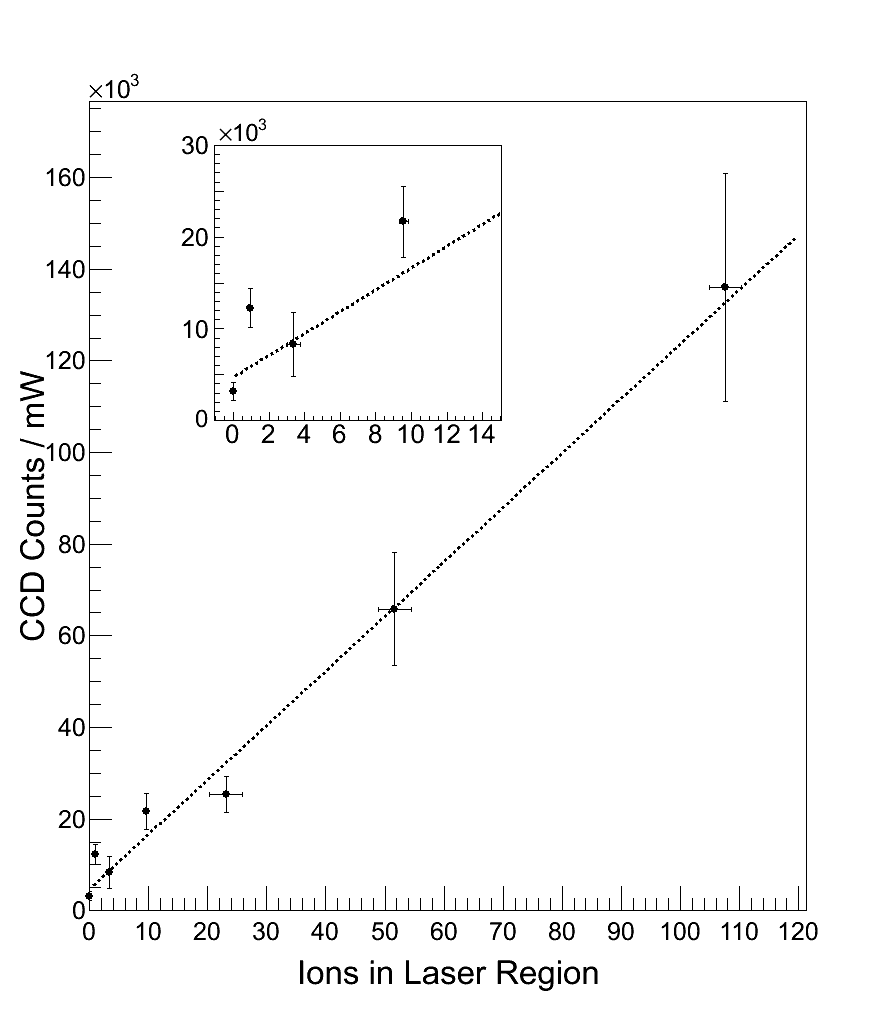
\includegraphics[width=.99\textwidth]{figures/fitgrouped_20150807_20150916_inset.png}
                \caption{\emph{\color{gray}Better may be all points with stat errors instead of combined points, and try adding other days too:  5-26, and something before that (and after?).  X errors should prolly just be systematic.}  Combined 2015-08-07 and 2015-09-16 with statistical errors.  \emph{\color{gray}Move y-axis title over.}}
\label{fig:lin}
\end{figure}

At low laser intensities, the 619-nm peak appears minor compared to the 577- and 591-nm peaks.  However, its much lower bleaching rate brings it to dominate over larger exposures, e.g. with the intensity of a focused laser at 0.01-0.1~mW over seconds or minutes.  Experiments imaging small numbers of Ba atoms in SXe in a focused laser region with the 619-nm peak were successful down to the single-atom level.

\begin{figure} %[H]
        \centering
                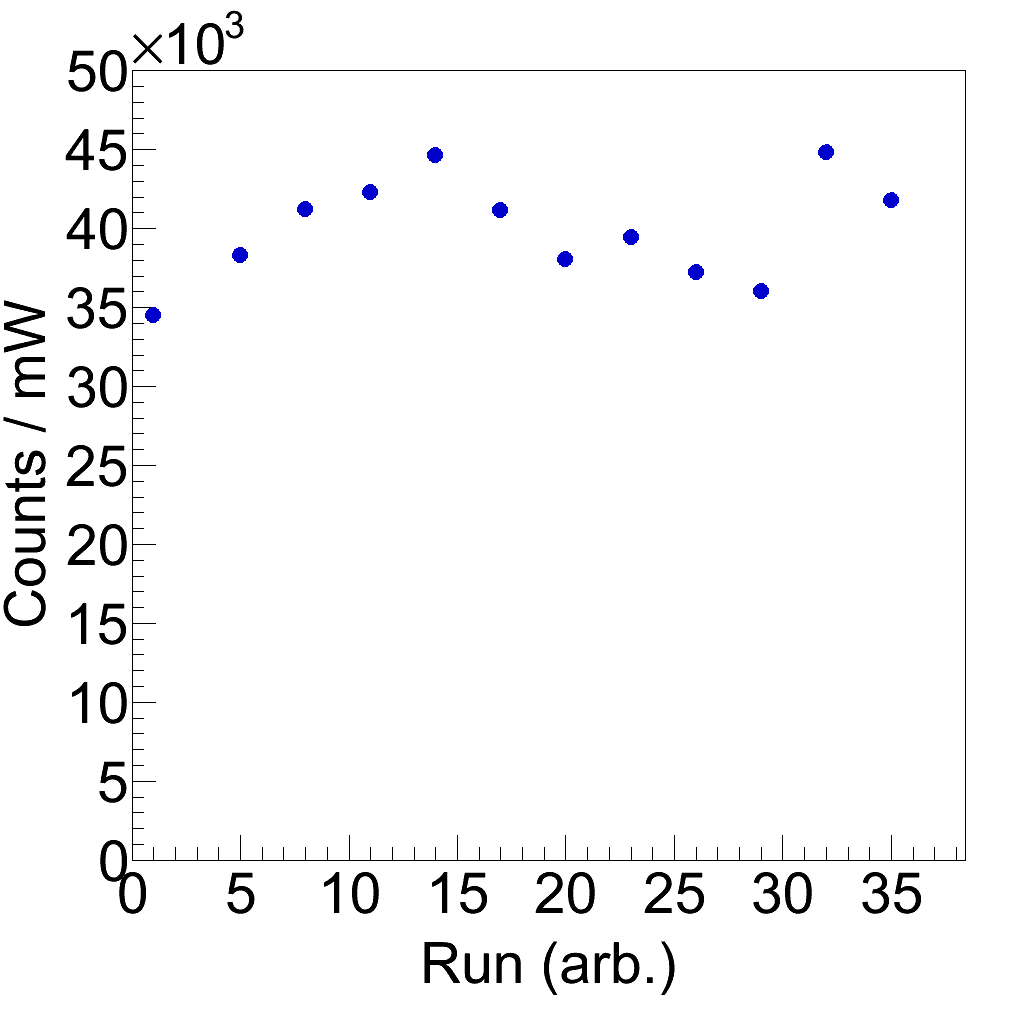
\includegraphics[width=.4\textwidth]{figures/xe_variation.png}
                \caption{}
\label{fig:xevar}
\end{figure}

An imaging experiment consisted of many different pulsed Ba\textsuperscript{+} deposits, each of which was evaporated after observation.  This procedure is described in \ref{sec:deposition}-\ref{sec:collection}.  A linear relationship between observed signal and ions deposited must be observed and repeated.  Frequent Xe-only deposits ware made, typically every three runs, to establish the local background.  The image of each deposit was analyzed by summing the counts of a 3-pixel$\times$3-pixel (15$\mu$m$\times$15$\mu$m) region centered on the laser spot in the SXe layer where it excites Ba atoms, i.e. at the top of the laser path in Fig. \ref{fig:imageexamp}.  A partial-bin integrator was implemented such that the 3-pixel$\times$3-pixel region could be centered on the peak center of each run, which typically varied by about half a micron between runs.  Summed counts vs. Ba\textsuperscript{+} ions deposited into the laser region is shown in Fig. \ref{fig:lin} for a combination of data sets from {\color{red}two} separate days \emph{\color{gray}maybe you want them separate (with each point having errors) by color to show agreement ... and try combining those other days.  It will require scaling for intensity difference (spher. abb.) and time, and remember different I$\times$t might give different efficiency.}  Each point has subtracted the averaged counts from the two surrounding Xe-only deposits.  Some variation in signal is observed, likely due to spatial drifting of the ion beam, as this variation was larger on days where larger beam drift was observed.  Nonetheless, a clear linearity in observed in signal vs. ions deposited, all the way down to single ions deposited.  Recall that the number of ions is an upper limit on the number of atoms in the 619-nm peak matrix site.  ``0-pulse" deposits are also made, wherein Faraday cup 3 is retracted for the 1-s period, but the ion beam remains deflected with no pulses.  This establishes the level of neutral Ba atoms making their way down the beam line from the source into the laser region.  Signal at the few-atom level is observed from these deposits.

\begin{figure} %[H]
        \centering
                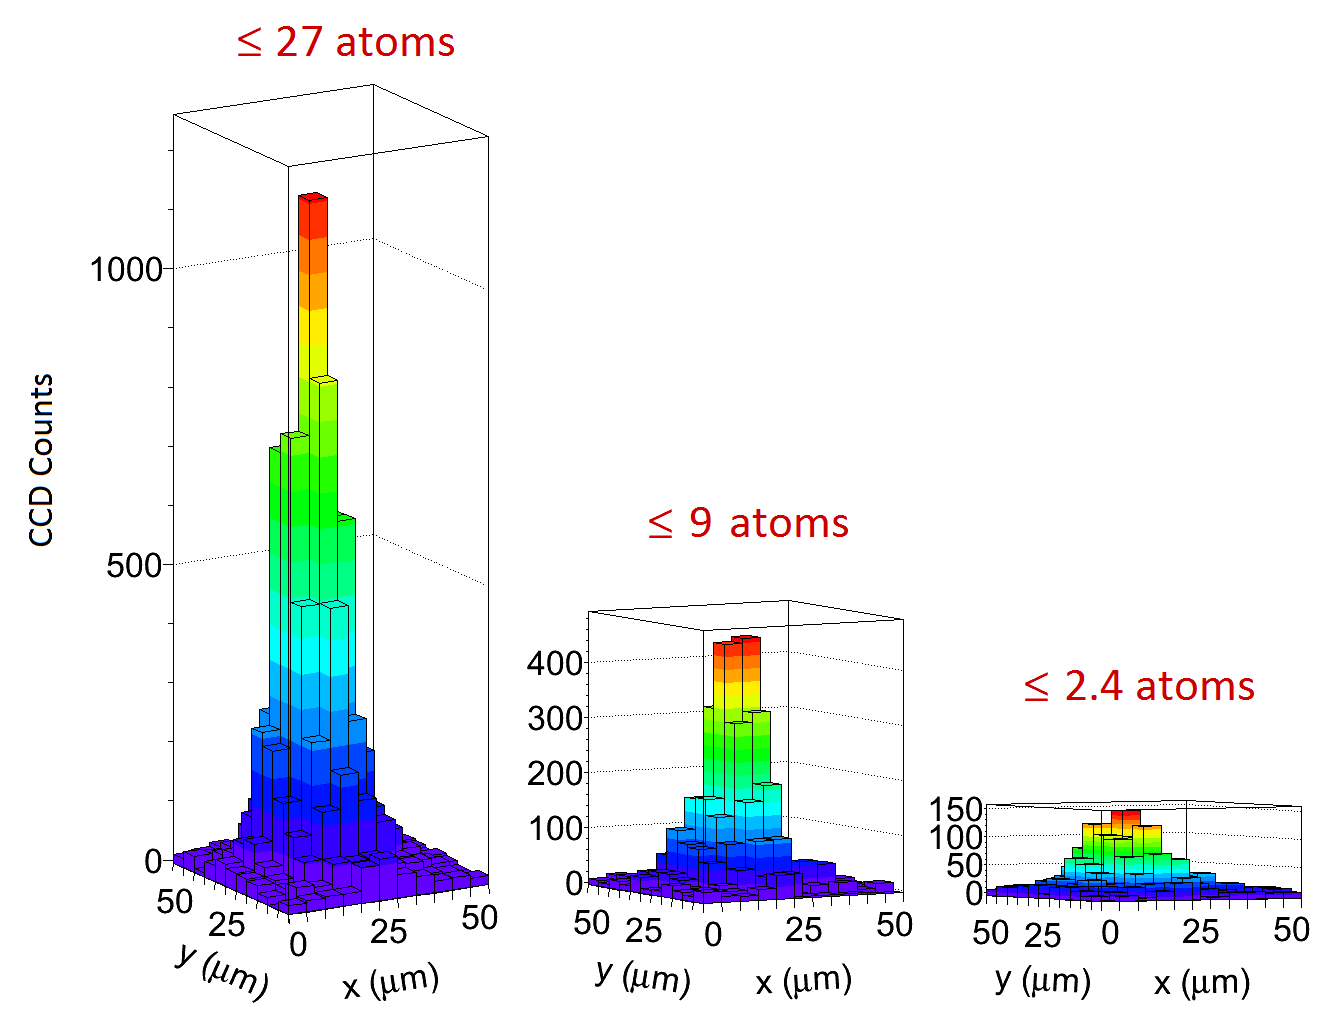
\includegraphics[width=.99\textwidth]{figures/train_20150807_v3_runs70_88_81_fromGiorgioFolder.png}
                \caption{\color{red}should:  1) have more than this, 2) do pixel (5micron) on axis like others, 3) have same-looking phi angle on all}
\label{fig:train}
\end{figure}

\begin{figure} %[H]
        \centering
                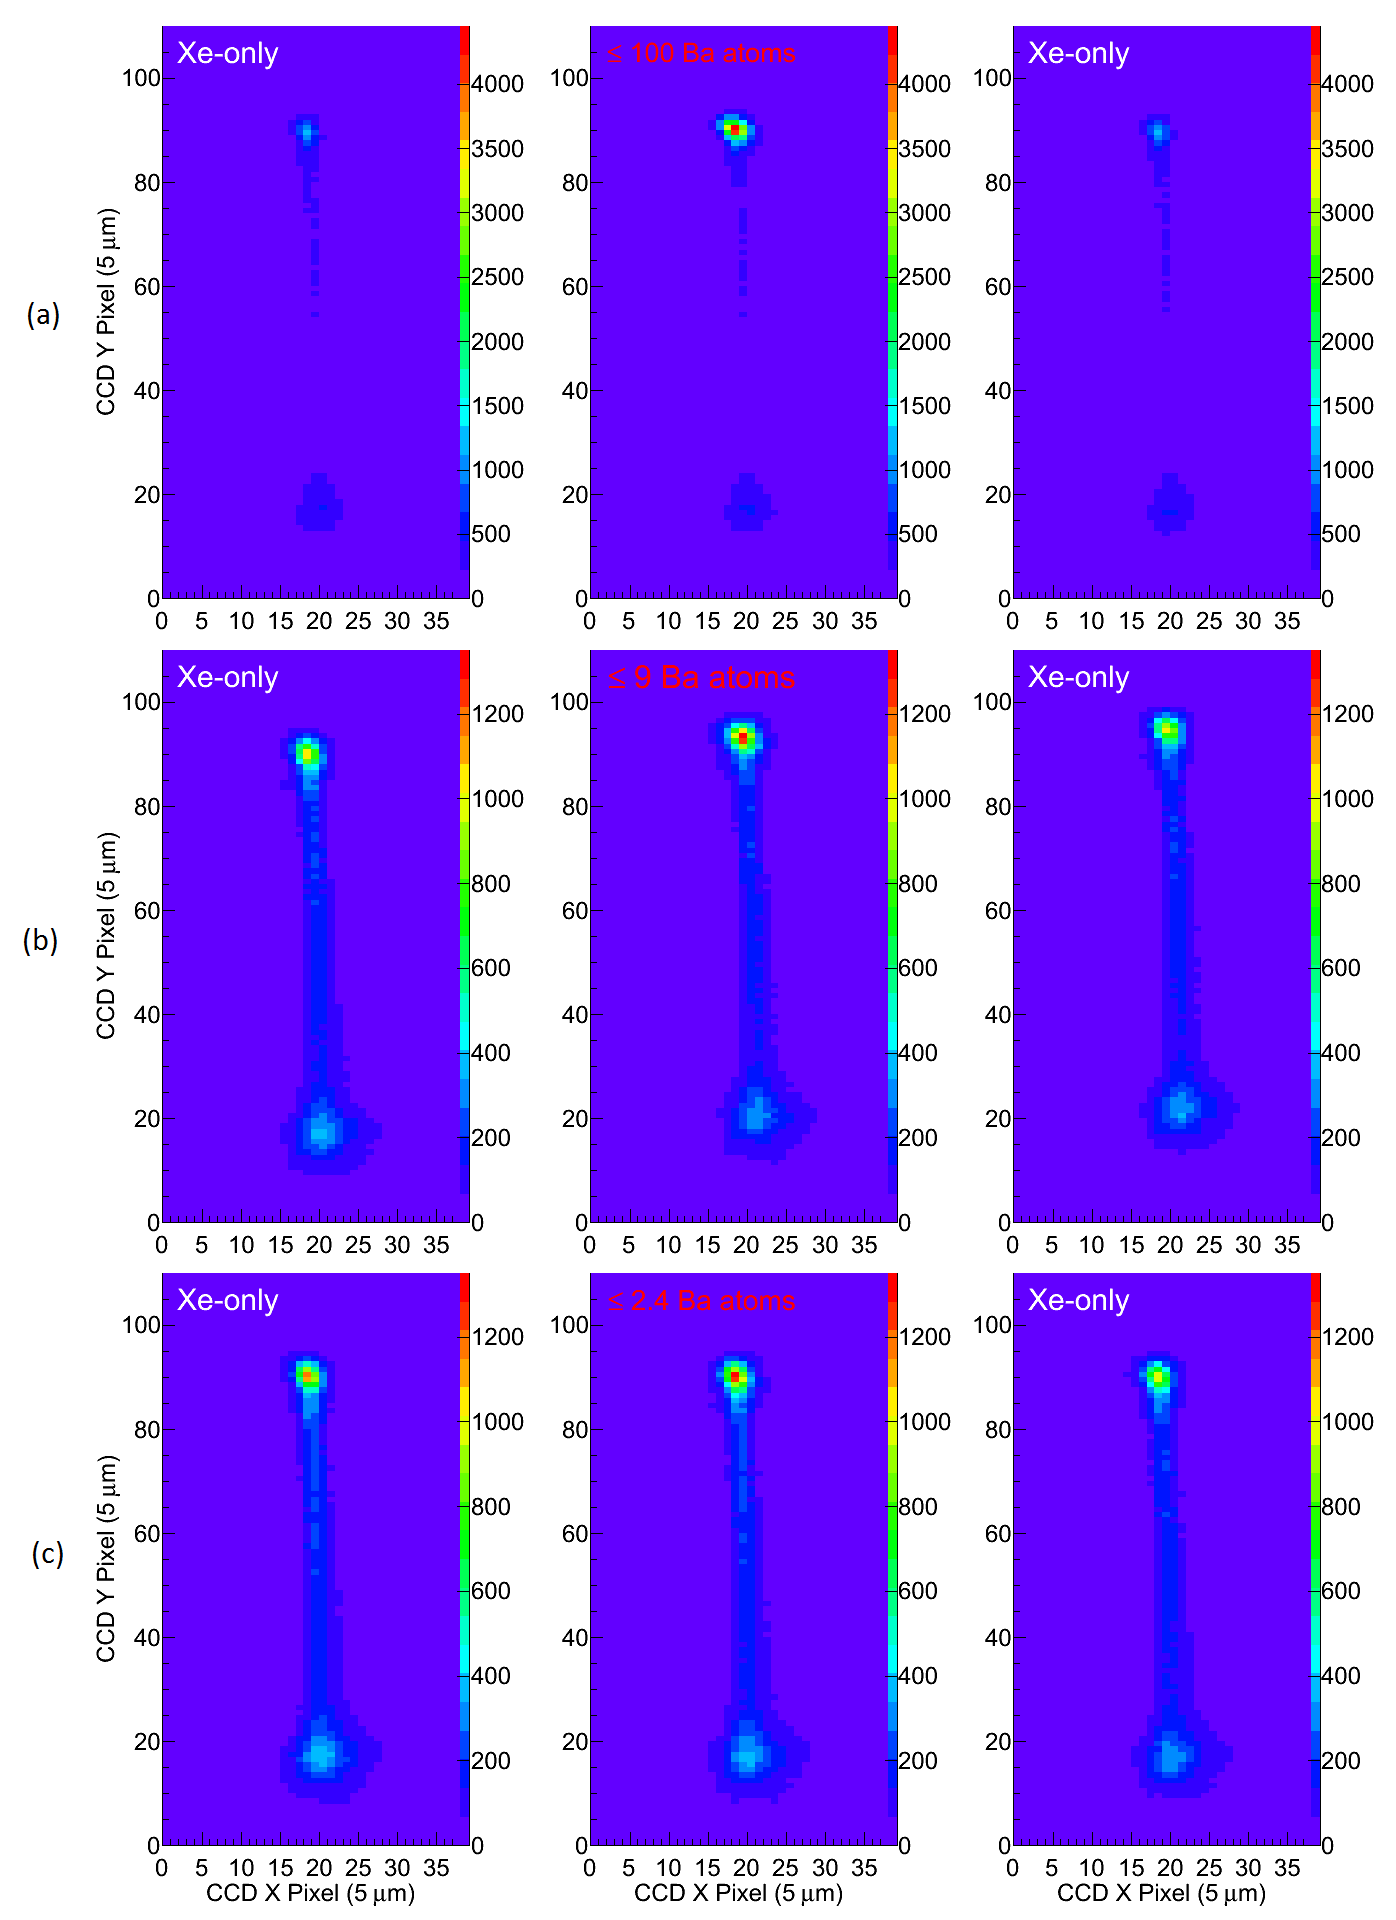
\includegraphics[width=.95\textwidth]{figures/xebaxe.png}
                \caption{Raw images of three Ba\textsuperscript{+} deposits yielding (a) $\leq 100$, (b) $\leq 9$, and (c) $\leq 2.4$ Ba atoms, with their preceding and succeeding Xe-only deposits.}
\label{fig:xebaxe}
\end{figure}

Variation in the background level, dominated by the surface background, is shown in Fig. \ref{fig:xevar}.  Variation was most likely caused by drift of the laser position on the window, to regions of different historical bleaching.  Local variations are at the single-atom signal level, however positive signal after subtraction, even at the single-atom level, demonstrates that this variation is sufficiently low.

Xe-only images were also directly subtracted to produce images of 619-nm Ba fluorescence.  In cases where the image has shifted slightly between runs, a binning redistribution was applied to do sub-pixel image shifting for better subtraction, though images which did not require this were preferred.  619-nm fluorescence images for several deposits of varying numbers of atoms are shown in Fig. \ref{fig:train}.  

It is important to note that no Ba signal is left behind after a sample is evaporated, even for large Ba\textsuperscript{+} deposits.  Raw images (pedestal-subtracted) of Ba\textsuperscript{+} deposits and their preceding and succeeding Xe-only deposits are shown in Fig. \ref{fig:xebaxe} for several runs.  The lack of historical buildup of Ba is important for the implementation of this method of Ba tagging on a probe in nEXO.

\subsection{Further Checks on 619-nm Peak}
\label{subsec:619identification}

The 619-nm peak, as well as the 670-nm peak, was attributed to neutral Ba by a few further tests.  A large Ba\textsuperscript{+} deposit is compared to a deposit made with the Ba getter in Fig. \ref{fig:ArVsBa}.  The 619-nm and 670-nm peaks were observed with both sources, and since the getter produces only neutral Ba, they were attributed to neutralized ions in Ba\textsuperscript{+} deposits.  Observation of the fluorescence with two different types of Ba sources is itself positive.  In addition, observation of the fluorescence with the low deposit energy of the getter may bode well for the prospect of grabbing on a probe in LXe.  Observation of a large deposit of Ar\textsuperscript{+} in SXe is also shown in Fig. \ref{fig:ArVsBa}.  The lack of fluorescence further disfavors a matrix-damage-related source of the fluorescence, such as color centers.  Finally, to rule out the possibility that the signal in Ba imaging experiments is due to passed wavelengths far from the 620-nm band-pass region, e.g. infrared, imaging experiments of Ar\textsuperscript{+} deposits in SXe were performed with both pulsing and continuous ion beams.  The same 620-nm band-pass filter was used, as well as the same focused 570-nm laser, to be similar to Ba\textsuperscript{+} 619-nm imaging experiments.  Summed counts from these deposits were consistent with background, as shown in Fig. [fig Ar+ pulse images].

\begin{figure} %[H]
        \centering
                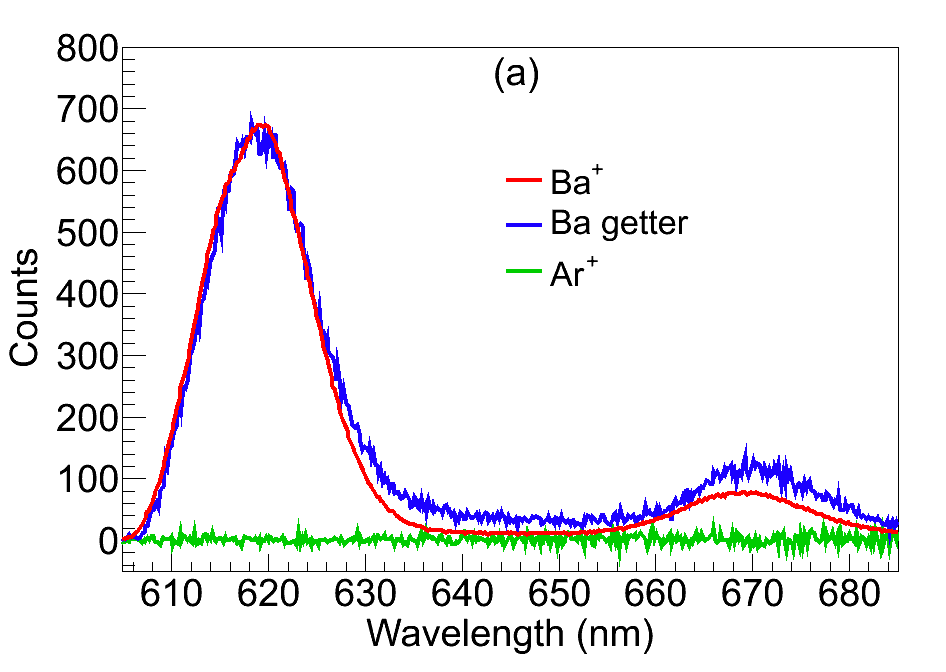
\includegraphics[width=.5\textwidth]{figures/Ar_vs_Ba.png}
                ~
                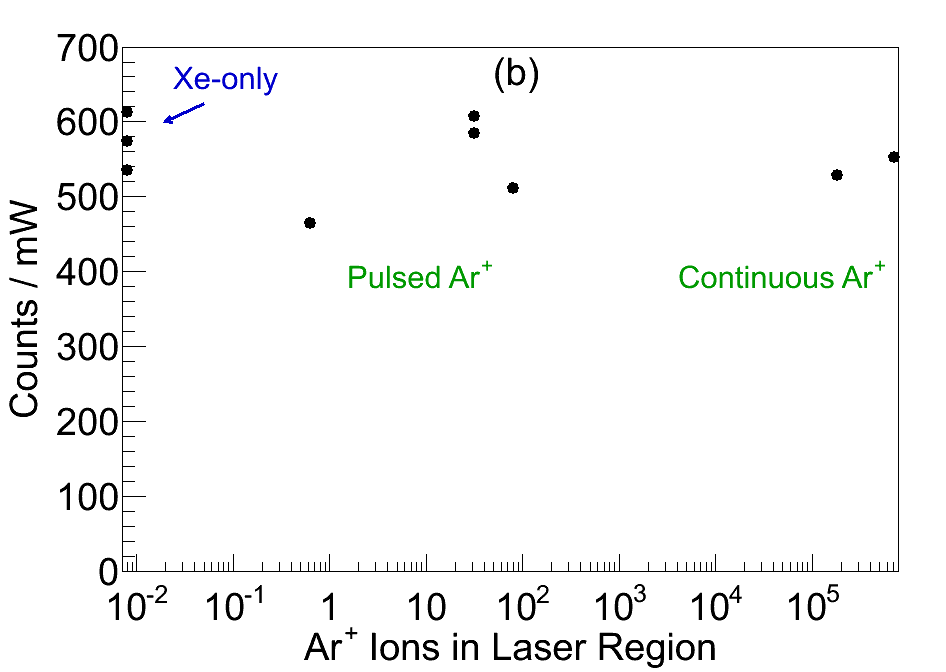
\includegraphics[width=.5\textwidth]{figures/ArImaging.png}
                \caption{}
\label{fig:ArVsBa}
\end{figure}

\emph{\color{gray}Whatever you did with the extra-filter-pass check (IR etc.) ... and was there something else?}

%at one point youthought leak rate dependence could go here

\section{Scanned Images}
\label{sec:scanning}

\section{Candidate Ba\textsuperscript{+} Lines/Blue Excitation}
\label{sec:BaPlus}

Since the fraction of neutralization of Ba\textsuperscript{+} deposited in SXe is not known to be 100\%, in this system but particularly in future tests of grabbing out of LXe, detection of single Ba\textsuperscript{+} in SXe is still of interest.  Preliminary studies of fluorescence from Ba\textsuperscript{+} deposits were performed by blue laser excitation with the C480 dye laser.

11~K vs 50~K (look back)?  I think so... so, you might start with Shon's lines, and then say that, similar to with Ba, more was found with 50~K deps (right?), and then talk about excitspec, and then get into the 530/630 identical excitspec as well as bleaching, and so say they are the candidates.  others are unidentified.

Mention 520~nm peak.

BaHx peaks -- discovered/identified by Shon, but further atributed to H by temp and leak rate (BaSpec).